
\documentclass [french]{sig-alternate-05-2015}
\usepackage{color}
\usepackage[francais]{babel}
\usepackage[utf8]{inputenc}
\usepackage{lmodern}
\usepackage[noend]{algpseudocode}
\usepackage{subcaption}
\usepackage{subfig} 
\usepackage{graphicx}
\usepackage[rflt]{floatflt}
\usepackage{mathrsfs}
\usepackage{multirow}
\usepackage{array}
\usepackage[rflt]{floatflt}
\usepackage{makecell}
\usepackage{usual}
\renewcommand\theadalign{cb}
\renewcommand\theadfont{\bfseries}
\renewcommand\theadgape{\Gape[3pt]}
\renewcommand\cellgape{\Gape[3pt]}

\begin{document}



\title{Un modèle pour prendre en compte les relations interpersonnelles dans les stratégies de dialogue}



\numberofauthors{3} 
\author{
\alignauthor Lydia Ould Ouali\\
       \affaddr{LIMSI}\\
       \affaddr{rue John von Neumann}\\
       \affaddr{91405 Orsay }\\
       \email{ouldouali@limsi.fr}
% 5th. author
\alignauthor Nicolas Sabouret\\
       \affaddr{LIMSI}\\
       \affaddr{rue John von Neumann}\\
       \affaddr{91405 Orsay }\\
       \email{sabouret@limsi.fr}
        \and
% 6th. author
\alignauthor Charles Rich\\
       \affaddr{WPI}\\
       \affaddr{Worcester Polytechnic Institute}\\
       \affaddr{Worcester, MA, USA}\\
       \email{rich@wpi.com}    
}


\maketitle
\begin{abstract}

\end{abstract}


\keywords{Relation interpersonnelle;negociation coopérative, dialogue social}

\section{Introduction}


%La modélisation d’agents conversationnels connaît un véritable essor dans différents domaines applicatifs où l'agent est muni d'un système de dialogue lui permettant de jouer différents rôles tels que  le rôle de compagnon \cite{sidner2013always} ou encore de conseiller \cite{bickmore2005s}. 
Les agents conversationnels animés (ACA) sont utilisés dans de nombreuses applications de l'assistance utilisateur [ref] au compagnon artificiel \cite{sidner2013always, riviere2014aca} en passant par le patient virtuel \cite{annesysteme} ou le recruteur virtuel \cite{jones2012affective}. Tous ces ACA sont munis d'un système de dialogue, plus ou moins élaboré; leur permettant de déterminer quelle phrase choisir en fonction de la situation observée.
\par Les systèmes de dialogues existants peuvent être divisé en deux catégories: les systèmes de dialogue orienté tâches et les systèmes de dialogue sociaux. Les systèmes de dialogues orienté tâches apparus en premier: les dialogues se centrent exclusivement sur la collaboration avec l’utilisateur pour satisfaire des tâches communes \cite{allen1995spoken, allen1996robust}. Cependant, un certain nombre de recherches ont montré que l’aspect social ne peut être ignoré dans un dialogue, car ce dernier est social par définition \cite{markopoulos2005case}. Par ailleurs, \cite{moon1998intimate} a démontré que les utilisateurs préféraient interagir avec des agents dotés d'aptitudes sociales qui lui permettraient de construire une relation sur le long-terme avec l'utilisateur \cite{bickmore2005establishing}. Par conséquent, les chercheurs s'intéressent de plus en plus aux systèmes de dialogues sociaux qui prennent en compte en plus des tâches à satisfaire, l'aspect social de la conversation dans la mise en œuvre de systèmes de dialogues. Néanmoins, il existe encore peu de recherches qui s’intéressent a une modélisation explicite et dynamique de la relation sociale entre l’agent et l’utilisateur (c.-à.-d. qui évolue au cours de l'interaction). Les travaux existants se sont limités à une modélisation qui vise a améliorer la collaboration de l’agent et l'utilisateur sur une interaction limitée dans le temps. Dans le cadre d'une interaction sur long-terme (voir section \ref{RW}), une modélisation explicite du comportement social de l’agent doit être considérée, car cette dernière influence le dialogue directement, en terme de contenue et de stratégies mises en place par l’agent pour satisfaire ses buts \cite{bickmore2012empirical}.

\par La modélisation des comportements sociaux a été largement étudiée en psychologie sociale, plusieurs travaux ont analysés les différentes dimensions qui peuvent affecter le comportement social dans le cadre d’une interaction humain/ humains. Ces notions peuvent être adaptées et utilisées pour le cas d’une interaction humain agent.

 \par En outre le dialogue social est défini pas \emph{Laver}\cite{laver1981linguistic} comme un processus d'échange de préférences et d'opinions sur un sujet de conversation. Cet échange de préférences peut conduire les interlocuteurs à mener une négociation - sur leurs préférences - afin de trouver un compromis qui arrangerait les deux participants. Par exemple, deux interlocuteurs qui cherchent un restaurant où dîner à Paris. Ce type de négociation est nommé \emph{négociation coopérative}. Nous pouvons donc considérer un dialogue social comme un processus de négociation coopérative sur les préférences, où les stratégies employées par les interlocuteurs pour présenter leurs préférences sont directement affectées par leurs perceptions de la relation interpersonnelle.

\par Dans cette optique, nous proposons dans cet article d'étudier l'impact des relations interpersonnelles sur les stratégies de dialogue employées par interlocuteurs spécialement dans le cadre d'une négociation coopérative. L'article sera structuré comme suit. La section \ref{RW} reprend les les travaux autours de notre thématique. La section \ref{contribution} sera dédiée à la présentation de notre modèle dialogique préliminaire ainsi que son implémentation. Les perspectives et futurs travaux, plus spécialement l'évaluation du système proposée seront discutés dans la section \ref{conc}.

\section{Travaux connexes}
\label{RW}
  
La modélisation d'un dialogue social consiste à concevoir un modèle de conversation où les buts interpersonnels sont mis en avant et les buts orienté tâches, s'ils existent, sont mis en arrière plan \cite{bickmore2005social}. Dans le cadre d'une négociation coopérative dans un dialogue social, le but social influence la négociation et la stratégie utilisée. Il existe déjà dans la littérature des travaux sur la négociation coopérative dans le dialogue. Par exemple \cite{amgoud2000arguments, daskalopulu1998handling} qui ont mis en œuvre des modèles formels de dialogue où les agents sont capables de négocier et même d'argumenter sur leurs choix de préférences. Cependant, ces travaux négligent l'aspect social du dialogue dans la conception des stratégies de négociation. En outre, il a été prouvé que les relations sociales affectent directement le comportement des interlocuteurs \cite{bickmore2000weather, bickmore2005establishing, moon1998intimate, nass2000does} et par conséquent leurs stratégies dans le dialogue. Par exemple, une personne dominante exprime plus facilement ses préférences et argumente contrairement a une personne soumise. 

\subsection{ACA sociaux}

\par Il existe dans la littérature des  ACA sociaux  qui arrivent à modéliser leurs relations avec l'utilisateur et la gérer afin d'adapter leur comportements dans la conversation. Le robot \textit{Autom} \cite{kidd2005sociable} qui est placé dans les maisons des utilisateurs pour une intervention sur le long terme. Le robot s'intéresse principalement à trois facteurs de relations avec l'utilisateur: \textit{l'engagement, la confiance et la motivation} qu'il construit sur trois étapes: la prise de connaissance, la construction des relations et enfin la maintenance de la relation. Le système dispose d'un nombre limité d'actes de langage pour  entretenir sa relation avec l'utilisateur. \textit{FitTrack} \cite{bickmore2005s} qui utilise un large éventail de techniques tirées de la psychologie sociale des relations. Tous ces comportements sociaux ont pour but d’accroître le lien social avec l'utilisateur au cours de l'intervention.
 Cependant, les comportements sociaux ne sont pas généré dynamiquement. Ils sont préalablement codé dans le dialogue de l'agent qui est basé sur une machine d'états fini et apparaissent selon un calendrier pré-défini. Ainsi, le modèle relationnel évolue implicitement dans le temps. \textit{REA} \cite{bickmore2005establishing} est un agent incarné grandeur nature qui joue le rôle d'un agent immobilier. Le planificateur décide dynamiquement de choisir entre le dialogue social ou sur des un dialogue orienté tâches. Un des facteurs de choix de dialogue est basé sur une évaluation de la relation actuelle avec l'utilisateur. La relation a été modélisé en utilisant un modèle tridimensionnel \cite{svennevig2000getting} et une dimension de \textit{confiance} a été ajoutée au système pour améliore les performances. La mise à jour des relations est basée sur le nombre et le contenu des mouvements de conversation.
\textit{AlwaysOn} \cite{sidner2013always} est un agent incarné pour une interaction avec les personnes âgées sur un long terme. Ce système s'intéresse à l'étude de l'engagement et des relations qui se créent avec l'utilisateur au cours des interactions. En effet, il dispose d'un planificateur qui décide quelle activité suggérer à l'utilisateur en fonction de l'évolution de la relation de \textit{proximité}.L'interaction se fait via un dialogue textuel et l'utilisateur choisit sa réponse à partir d'un menu.


\par Notre travail s'inscrit dans la continuité de ces travaux dans le sens où nous modélisons un agent conversationnel qui puisse percevoir sa relation avec l'utilisateur et adapter ses stratégies de négociation et dialogue en fonction de sa perception de la relation. 

\subsection{Formalisme des relations interpersonnelles}
\label{RI}
 Il existe de nombreuses représentations des relations interpersonnelles dans la littérature. Cependant, la représentation dimensionnelle demeure la plus courante. Elle consiste à projeter les relations dans un cercle de dimensions \emph{(c.f modèles de Wiggins)}. Par conséquent, toute relation peut être située et évaluée dans cet espace dimensionnel \textit{continu}. Un des modèles les plus connus est celui de Svennevig \cite{svennevig2000getting} qui divise les relations interpersonnelles sur quatre dimensions. La dominance, familiarité, affect et solidarité. Nous nous intéressons plus particulièrement à la relation de dominance, qui est un comportement social typique qu'on peut observer dans les interactions humaines \cite{dunbar2005perceptions}. On retrouve différentes définitions de la relation de dominance dans la littérature mais elles convergent toutes à définir la dominance comme le pouvoir d'influencer le comportement d'autrui afin d'asseoir son autorité. La position de dominance en terme de relation interpersonnelle peut être manifeste \cite{dunbar2005perceptions} dans laquelle l'assertion de dominance manifestée chez un interlocuteur rencontre forcement  l'acquiescement de l'autre \cite{rogers1979domineeringness}. Elle peut aussi être latente \cite{komter1989hidden} où l'interlocuteur dominant n'a pas conscience de sa position de dominance. Ce genre de comportements peut affecté l'interaction de manière positive ou négative. L'apport positive consiste a permettre par exemple d'entretenir la conversation, orienter la tâche courante de l’interaction, prendre des décisions rapides et efficaces et définir des conclusions. Cependant, ce même comportement peut affecter l’interaction de façon négative où la personne dominante peut étouffer l'autre et ne pas lui laisser la possibilité d'exprimer ses opinions. Cette expression verbale de la dominance peut être perçue comme offensive et injustifié par l'autre et peut mener a des conflits dans le dialogue si les deux interlocuteurs sont dans une position de dominance avec des opinions différentes.
\par Plusieurs approches existent pour détecter les comportements de dominance dans l'interaction. Ces indicateurs peuvent être soit verbaux ou non verbaux. Les indicateurs non verbaux peuvent être vu dans les expressions faciales tels que le regard, le ratio de dominance visuel \cite{dunbar2005perceptions} qui ont montré qu'un grand ratio de dominance visuel est corrélé avec une grande perception de dominance. Le contrôle de la posture et les gestes sont aussi perçue comme une comportement dominant. Carney, Hall, and LeBeau (2005)  ont montré que les personnes dominantes avaient tendance à plus utiliser les gestes tels qu'une poignée de main ou bien une plus grande fréquence "invasive touch". Les indicateurs verbaux incluent la fréquence d'intervention dans l'interaction, leurs durée (le nombre de mots utilisés et répétés) \cite{dunbar2005perceptions}, l'expression des opinions et la critique, suggestions, demandes, réactions, ignorance, etc \cite{zablotskaya2012relating} et enfin la capacité d'interrompre la conversation et changer le sujet de conversation.

%{\color{red} Ajouter une fin de section: comment cette dimension va être utilisé dans notre modèle (ex:  nous avons remarqué que la relation de dominance permettait l'apparition de comportements qui nous semblent intéressants à reproduire dans un agent conversationnel)}

\section{Contributions}
\label{contribution}

\par Afin de réaliser nos objectifs, nous avons d'abord enregistré des dialogues entre deux personnes afin d'observer leurs comportements dans un cadre de dialogue social. 
Pour l'étude de ces comportements, nous avons annotés et analysé les dialogues. Cette étude nous a livré un ensemble de comportements  que nous avons ensuite reproduit dans des jeux de dialogues dans le modèle D4G utilisé au sein de la plate-forme de dialogue Disco \cite{rich2009building}. 
 Les informations collectées grâce l'observation des comportements humains nous a guidés dans la conception de notre modèle dialogique avec une modèle mental de l'environnement de l'agent, et un modèle lui permettant de mener une négociation coopérative. 
En parallèle, nous avons modélisé un module de communication comportant cinq actes dialogiques qui lui permettent de dialoguer et négocier. Nous présenterons dans cette partie nos travaux menés ainsi qu'une première implémentation de ce modèle.

La première étape de notre contribution a pour but de mieux comprendre les comportements liés à la dominance qui peuvent émerger durant une négociation coopérative durant un dialogue. Nous avons donc enregistré deux dialogues dans lesquels les interlocuteurs avaient pour but de trouver un restaurant où dîner sur paris. Trois hypothèses tiré de la littérature (voir section \ref{RI}) ont guidé l'analyse de ces comportements: 
\begin{itemize}
\item \textbf{H1:} Un interlocuteur dominant a tendance à influencer le dialogue (capacité de diriger le dialogue).
\item \textbf{H2:} Il prends la parole plus souvent et est capable d'exprimer explicitement ses opinions.
\item \textbf{H3:} Un interlocuteur moins dominant chercherait un compromis entre les deux. 
\end{itemize}
 Les dialogues enregistrés ont ensuite étaient annoté et analysé en se basant sur les travaux de Sidner \& Grosz \cite{grosz1986attention}. Nous avons effectué une analyse de \textit{la structure linguistique}  en décomposant le dialogue en segments de dialogue (DS)  et chaque DS a était analysé afin d'extraire son but qui participait à la satisfaction du but global. cette étape est nommée l'analyse de \textit{la structure intentionnelle}. Les résultats de cette analyse sont expliqué ci-dessous: 

\begin{itemize}

		\item  La segmentation du dialogue en DS nous a permis d'extraire le processus que suivaient les interlocuteurs dans l'exécution de la tâche  ``trouver un restaurant''. En effet, les interlocuteurs abordait systématiquement le type de la cuisine, l'ambiance, le prix, et la localisation. 
		\item L'analyse intentionnelle nous a permis d'identifier les buts communicatifs et buts internes des interlocuteurs. Par exemple, détecter un comportement dominant dans le nombre de fois où il initie un nouveau sujet de conversation, le nombre de prise de paroles, ainsi que la fréquence d'initiation de DS et la fréquence de propositions, l'argumentation ... ), qui nous a permis d'analyser l'évolution de la relation de dominance dans ces dialogues. 
		\item Identification d'actes de langage récurrents dans les dialogues qui nous ont aidé dans la définition d'acte de dialogue pour notre agent.	
	
\end{itemize}
\par Cette analyse nous a aidé a mieux cibler notre contribution, à savoir étudier l'impact de la relation de dominance dans les stratégies de dialogue.



\subsection{Modèle formel du dialogue}
\par Le modèle proposé vise à concevoir un agent conversationnel capable mener une négociation coopérative sur un sujet de conversation sociale et être capable d'adapter ses stratégies de dialogue a sa perception de sa relation interpersonnelle avec l'utilisateur. L'architecture proposée (illustré dans
% la \fig{modele} )
 se compose de trois principaux modules: un \textit{état mental} regroupant les préférences de l'agent et celles de l'utilisateur, un \textit{module de communication} comprenant les actes de langages que l'agent utilise pour dialoguer et enfin un module qui sauvegarde le \textit{contexte du dialogue} à savoir l'historique des informations échangées durant le dialogue (en termes de préférences et propositions échangées). Nous présentons dans cette section chaque module.

%\begin{figure}
%	\fbox{	\centerline{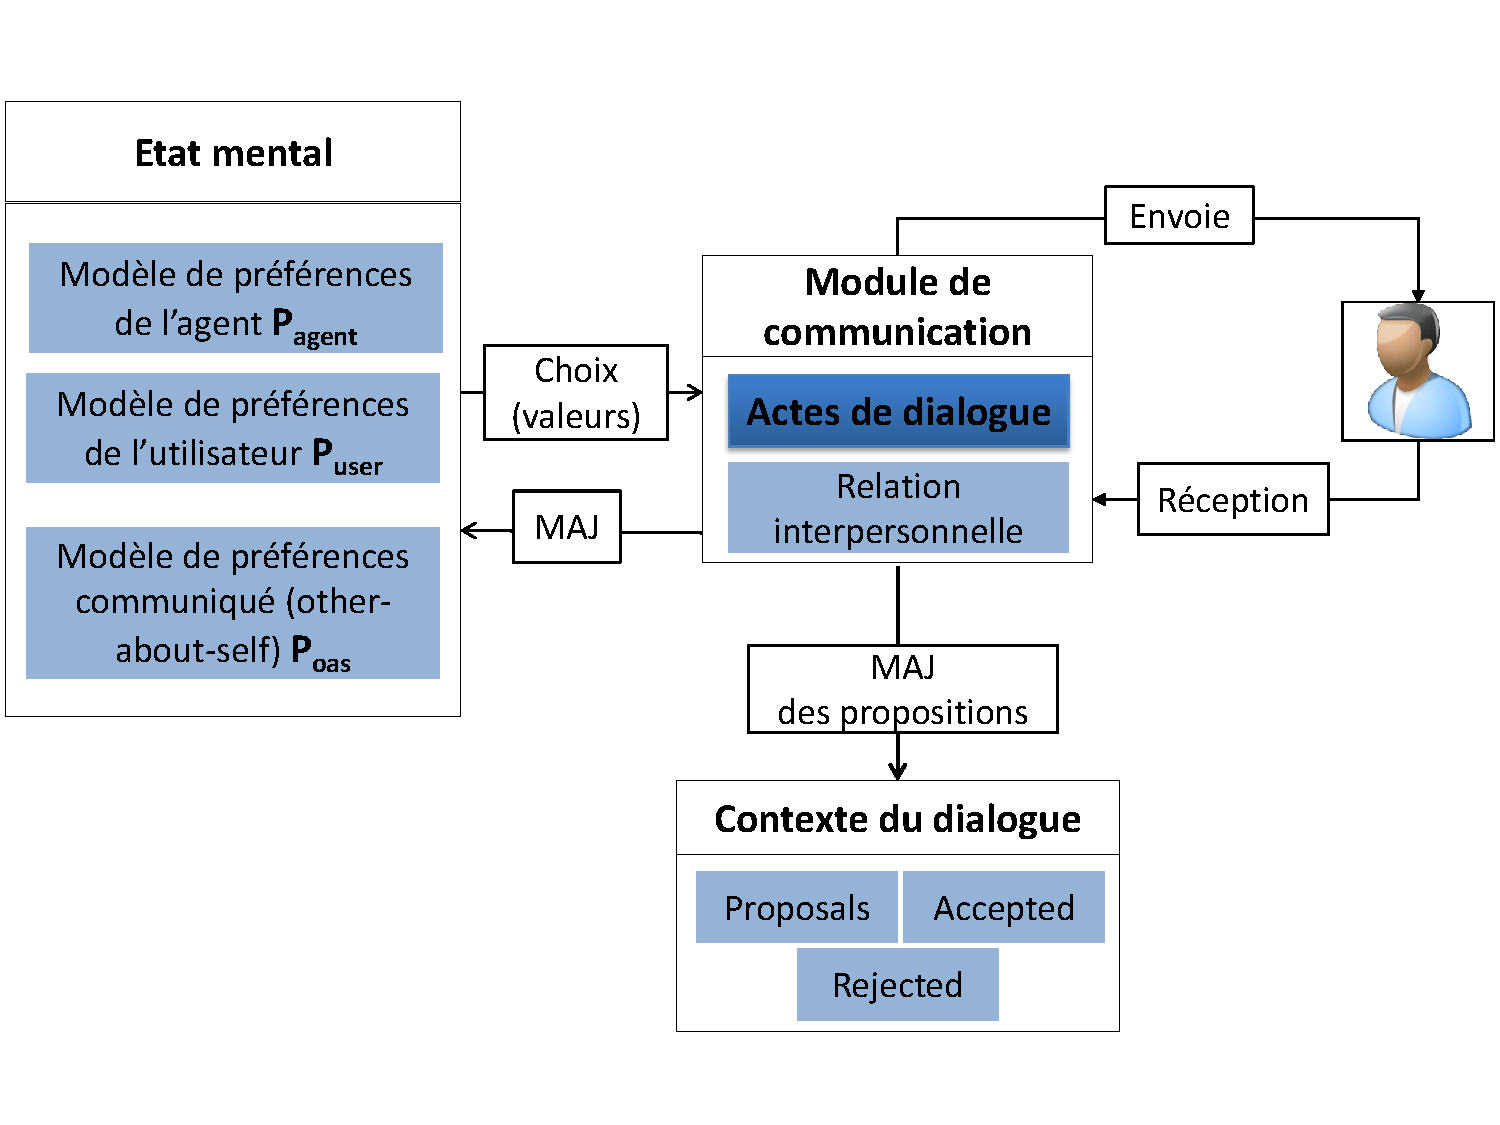
\includegraphics [width=4in]{figs/modele}}}
%	\vskip 8pt
%	\defig{modele}{Architecture du modèle de dialogue.}
%\end{figure}

\subsubsection{L'état mental}
\par Mener une négociation coopérative sur un sujet définis implique un processus décisionnel de la part des interlocuteurs  où les préférences de chacun sont censées régir ce processus décisionnel. Par conséquent, l'agent a besoin d'une modélisation formelle de cet environnement, à savoir ses préférences, ainsi que celles de l'utilisateur. Nous notons donc
 \begin{itemize}
 	\item  $\mathcal{P}_{self}$ le modèle de préférences de l'agent.
 	\item $\mathcal{P}_{other}$ le modèle de préférences de l'utilisateur que l'agent aura acquis durant le dialogue.
 	\item De plus; l'agent conserve les préférences qu'il communique à l'utilisateur durant la négociation (un module de la théorie d'esprit) qu'on note $\mathcal{P}_{other-about-self}$.
 \end{itemize}

% \par Dans ce qui suit, nous présenterons le modèle formel de préférences utilisé pour la représentation de l'état mental de l'agent.

\par \textbf{Le domaine de préférence :}
Le processus décisionnel d'une négociation  doit aboutir au choix d'une \emph{option} parmi un ensemble d'options qu'inclut le thème de la négociation (et donc de la conversation). Par exemple, pour une négociation sur le thème des ``Restaurants'', l'ensemble des options à choisir est l'ensemble des restaurants que les interlocuteurs connaissent.
 On note donc $\mathcal{O}$, l'ensemble des options définis pour un thème de négociation donnée. Les options sont définit avec un ensemble de critères qui reflètent leurs caractéristiques. Par exemple, les critères de choix d'un restaurant sont \{la cuisine, le prix, l'ambiance, la localisation\}. Nous notons $\mathcal{C}$ l'ensemble des critères des options définis dans $\mathcal{O}$.
 \par De plus, chaque critère a son domaine de valeurs \emph{D$_c$}. Par exemple, le domaine de valeurs du critère de la cuisine est noté $\emph{D}_{cuisine}$ = \{Chinois, Italien, Indien...\}.

\par Par conséquent chaque option $O\in \mathcal{O}$ définit une valeur pour chaque critère : 
$O = \{c_1=v_1,..., c_n=v_n\}$ avec $c_i \in \mathcal{C}, \forall i \in [1,n]$ et $v_i\in \emph{D}_{c_i}$, où $\{v(c,O) \in \emph{D}_{c} / \forall O \in \mathcal{O}, \forall c \in \mathcal{C}\}$ est la valeur \emph{objective} du critère $c$ attribué à l'option $O$. 
%La valeur objective d'un critère est indépendante des préférences; les interlocuteurs affectent les mêmes valeurs au critères d'une option indépendamment de leurs préférences. 
Par exemple, Ginza est un restaurant japonais coûteux : $v(prix, Ginza) = couteux $ et $(cuisine, Ginza) = japonais$. 


\par L'agent est capable d'exprimer ses préférences sur ce domaine de connaissance avec une fonction de préférence. Nous définissons une préférence \emph{P} comme une relation \emph{transitive} et \emph{antisymétrique} définit sur un ensemble d'éléments \emph{A}, tel que:

\[ \left \{
\begin{array}{l}
\emph{P(a,b)} $ : \emph{b}  est préféré à $\emph{a}. \emph{ a,b} \in \emph{A}\\
\emph{P(b,a)} $:  \emph{a} est préféré à  $\emph{b}. \emph{ a,b} \in \emph{A}\\
$Sinon, aucune . $\\
\end{array}
\right .\]

Par exemple $P_{cuisine} (Italien, Japonais)$ signifie que l'agent préfère la cuisine japonaise à l'italienne. 

\par Nous définissons des variantes pour la notion de préférences:
\begin{itemize}
	\item  \emph{P(*,a)}  = \{$\forall$ \emph{x}$\in$\emph{A}, \emph{P(a,x)}\}, représente le fait que  \emph{a} est l'élément  \textit{le plus préféré} dans \emph{A}.
	\item Par opposition, \emph{P(b,*)} = \{$\forall$ \emph{x}$\in$\emph{A}, \emph{P(x,b)}\} signifie que \emph{b} est l'élément \textit{le moins préféré} dans l'ensemble \emph{A}. 
\end{itemize}

\par Cette représentation de la relation de préférence nous permet de construire une base de préférences nommé $\mathcal{P}_{self}$ dans laquelle il stocke ses préférences sur les critères de $\mathcal{C}$ et ses préférences sur les valeurs de chaque $ c \in \mathcal{C}$. 
%
%\par Notre but est de définir des préférences sur les options de la négociation.  Nous retrouvons dans la littérature plusieurs méthodes de calcul des préférences d'une option \cite{dodgson2009multi}. Ces méthodes nommées décision multi-critères calculent les préférences d'une option selon les performances de cette dernière sur l'ensemble des critères qui la définissent. Dans l'ensemble\cite{dodgson2009multi}, le calcul des préférences d'une option est fait par inférence à partir des préférences enregistrées sur les valeurs de ses critères. Cette inférence peut être réalisée grâce à différentes méthodes comme la fonction de somme pondérée \cite{yager2012ordered} ou encore les intégrales de Choquet \cite{chouquet1953}. \\
%
\par  \textbf{Processus décisionnel basé sur les préférences :} 
Afin de trouver une option qui satisfasse les préférences des deux interlocuteur, l'agent doit être en mesure de calculer ses préférences sur les différentes options dans $\mathcal{O}$. La relation de préférence entre deux options est calculée par inférence à partir de $\mathcal{P}_{self}$ dont les connaissances lui permettent d'inférer l'utilité de chaque option grâce a une fonction de décision multi-critères. 
Nous avons sélectionné pour notre modèle la fonction de somme pondérée \cite{yager2012ordered} qui offre une méthode pour agréger les préférences sur les valeurs de chaque  critère $c \in \mathcal{C}$ calculé individuellement afin d'obtenir un score d'utilité globale pour l'option.
 \begin{itemize}
 	\item On note donc $score(v)$ le score de $v \in \mathcal{D}_{c}$ qui représente le nombre des successeurs de  $v$  dans le modèle de préférence $\mathcal{P}_{self}$, ce qui signifie que $|\{ \forall x \in \mathcal{D}_{c} / P (x,v) \in \mathcal{P}_{self}\}|$.
 	\item $rang(c)$ le rang d'un critère $c \in \mathcal{C}$ qui est le score normalisé de $c$ calculé en triant les critères de $\mathcal{C}$ par ordre croissant de leurs scores.
 \end{itemize}
Par conséquent, calculer l'utilité d'une option grâce à la fonction de somme pondéré est effectué comme suit:

\[U(O) = \sum_{c_j \in \mathcal{C}}  rang_R(c_j) \times score\left( v(O, c_j) \right) \] 


\par La relation de préférence entre deux options est donc calculée en comparant leurs utilités. 
\[ P(O_1, O_2)  = \left \{
\begin{array}{l}
P(O_1, O_2)$ \textit{if}  $U(O_1) < U(O_2) \\
P(O_2, O_1)$  \textit{if} $U(O_1) > U(O_2)  \\
$  \textit{aucune n'est préférée}  $U(O_2) = U(O_1)\\
\end{array}
\right .\]

{\color{red}
Ajouter un exemple }
\subsubsection{Contexte du dialogue}
\par Durant le dialogue, les deux interlocuteurs échangent des informations sur leurs préférences et suggèrent des propositions pour le choix d'une option. par exemple, je préfère manger Indien ce soir, ou allons au restaurant Ginza ...

Afin de capturer ces informations, nous définissons les éléments suivants:
\begin{itemize}
	\item Une proposition est définie comme un tuple $Proposal$ $(Type, Valeur)$ où $Type$ est soit le thème de négociation par exemple ''Restaurant``, soit un critère $c \in \mathcal{C}$ et $Valeur$:
	\begin{itemize}
			\item Une option $O \in \mathcal{O}$ si $Type \in Topic$ 
			\item Une valeur de critère $v \in \emph{D}_c$ si $Type \in \mathcal{C}$
	\end{itemize}

	\item Afin de garder trace de toutes les propositions soumises durant le dialogue, nous définissons ces structures de données qui stockent une proposition à chaque cycle de vie. 
		\begin{itemize}
			\item $ Proposed$ est la liste de toutes les propositions ouvertes dans le dialogue.
			\item $ Rejected$  est la liste des propositions rejetées.
			\item $ Accepted$  est la liste des propositions acceptées. Il est a noté qu'il suffit qu'une option soit acceptée pour pouvoir clore la négociation. 
		\end{itemize}
\end{itemize}

\subsubsection{Sémantique des actes de dialogue}
\par Les agents communiquent en utilisant des actes de dialogues. Les messages sont considérés comme des actions durant le dialogue. Ils sont donc définis avec des préconditions et des effets qui mettent à jours l'état mental de l'agent. Il est à noter que les préconditions sont toutes optionnelles, car le choix d'un message dépend en premier lieu de la stratégie de l'interlocuteur (i.e perception de la RI). Les effets d'un message modifient l'état mental de l'agent  mais en aucun cas ne changent les préférences de l'agent $\mathcal{P}_{self}$. 
\par Nous avons définis un ensemble d'actes de dialogues illustrés dans le tableau \ref{tab: utt} qui sont assez génériques pour permettre à l'agent d'exprimer différentes préférences afin de participer de manière efficace dans la négociation. Par exemple, l'acte de dialogue "State.Preference" permet à l'agent d'exprimer une préférence sur n'importe quel domaine. Par exemple: \\ State.Preference$_{cuisine}(\textit{Japanese , Chinese})$ : ``I prefer japanese cuisine over Chinese''. 
L'expéditeur de cet acte doit avoir cette préférence dans son modèle. Il est a noter par ailleurs que l'effet de cet acte diffère selon le rôle de l'agent (expéditeur/récepteur). En effet, si l'agent est l'expéditeur de ce message, il aura à mettre à jour le modèle contentant les informations que l'utilisateur détient sur l'agent. En parallèle, si l'agent est le récepteur de ce message, il aura à mettre à jour ses connaissances sur les préférences de l'utilisateur

\begin{table*}
	
	\caption{\label{tab: utt} Sémantique des actes de dialogue}
	\begin{tabular} {|m{0.40cm}|m{4cm}|m{2cm}|m{2.5cm}|m{3cm}|m{2.5cm}|}
		
		\hline 
		N & \thead{Utterance} & \multicolumn{2}{c|} {\thead{Preconditions}  } &  \multicolumn{2}{c|} {\thead{Effects}  } \\
		\hline 
		1 & \makecell{State.Preference(\textit{$a,b$}):\\ ``I prefer $a$ over $b$''}& \multicolumn{2}{c|} {\makecell{ $(a,b)\in$ $\mathcal{P}_{self}$  \\ $(a,b) \notin$ $\mathcal{P}_{oas}$} }&\makecell{ \textit{(hearer case)} \\ $add((a,b)$, $\mathcal{P}_{other})$ } & \makecell{\textit{(speaker case)} \\ $add((a,b)$, $\mathcal{P}_{oas})$}  \\
		\hline
		2 & \makecell{Ask.Preference(\textit{$a,b$}):\\``Do you prefer $a$ to $b$'' ?}& \multicolumn{2}{c|} {\makecell{ $ (a,b) \notin \mathcal{P}_{other} $} }&
		\multicolumn{2}{c|} {\makecell{None} } \\
		\hline
		3 & \makecell{Propose(\textit{Proposal(T,V)}):\\``Let's choose  \textit{V}''}& \multicolumn{2}{c|} {\makecell{$ Proposal(T,V) \notin  Proposed$} }&\multicolumn{2}{c|} {\makecell{ $add(Proposal(T,V), Proposed)$ }} \\
		\hline
		4 & \makecell{Accept(\textit{Proposal(T,V)}):\\``Okay, let's choose \\ \textit{V} for \textit{T}''}& \multicolumn{2}{c|} {\makecell{$Proposal(T,V) \in Proposed$ \\ $ Proposal(T,V)\notin Accepted$} } & \multicolumn{2}{c|} { \makecell{$add(Proposal(T,V), Accepted)$\\$ remove(Value, Proposed)$}  }  \\
		\hline
		5 & \makecell{Reject(\textit{Proposal(T,V)}):\\`` Sorry, I would choice \\ something else.''}& \multicolumn{2}{c|} { \makecell{$Proposal(T,V) \in Proposed$ \\$Proposal(T,V)\notin Rejected$}  } & \multicolumn{2}{c|} {\makecell{ $add(Proposal(T,V),Rejected)$ \\$remove(Proposal(T,V), Proposed)$}} \\
		\hline
	\end{tabular}
\end{table*}

\subsection{Implémentation du modèle de dialogue}

\par Nous avons réalisé une première implémentation de notre système de dialogue avec un modèle générique de l'état mental qui permet à l'agent de mener une négociation dans un sujet de conversation donné. Un exemple sur le sujet des restaurants est déjà réalisé. Les actes de dialogue quand a eux sont implémenté avec le logiciel Disco \cite{rich2009building} qui supporte la création d'actes de dialogue ainsi que la génération d'arbres de dialogue.

\subsubsection{Présentation de Disco}
Disco est une implémentation d'un ``collaborative discourse manager'' inspiré d'une théorie de dialogue collaboratif comme Collagen.  Disco est un système qui permet la génération de dialogues orienté tâches pour lequel il utilise le formalisme des HTNs pour la gestion des tâches. implémenté avec le standard ANSI/CEA-2018.
Chaque tâche est définit avec des préconditions, des effets et des postconditions. 
\par De plus, Disco a été étendu avec un module génération d'arbres de dialogues afin de communiquer et collaborer avec l'utilisateur pour la réalisation des tâches. Ce module est nommé Disco for Games (D4g) et permet de définir des sémantiques d'actes de dialogue. D4g est déjà fourni avec un ensemble d'actes de dialogue. Cependant, nous l'avons étendu avec les actes de dialogues présenté dans la section \label{contribution} afin qu'il puisse supporter la négociation sur les préférences. 
\subsubsection{Génération de dialogue} 
 \par Le système de dialogue offre à l'utilisateur la liberté de choisir n'importe quel acte de dialogue pour son tour de parole. Par conséquent, l'agent doit être en mesure de produire une réponse adéquate qui respecte l'été mental courant ainsi que la RI perçue peu importe l'acte de dialogue généré par l'utilisateur. Nous avons implémenté des sous arbres de dialogue qui peuvent adapter la réponse de l'agent en fonction de  l'acte de dialogue choisi par l'utilisateur ainsi que son observation de l'environnement. Par exemple, les réponses que l'agent peut générer quand il reçoit un \emph{StatePreference} de la part de l'utilisateur sont présenté dans la \fig{state}.
 \begin{figure} [h]
 	\centerline{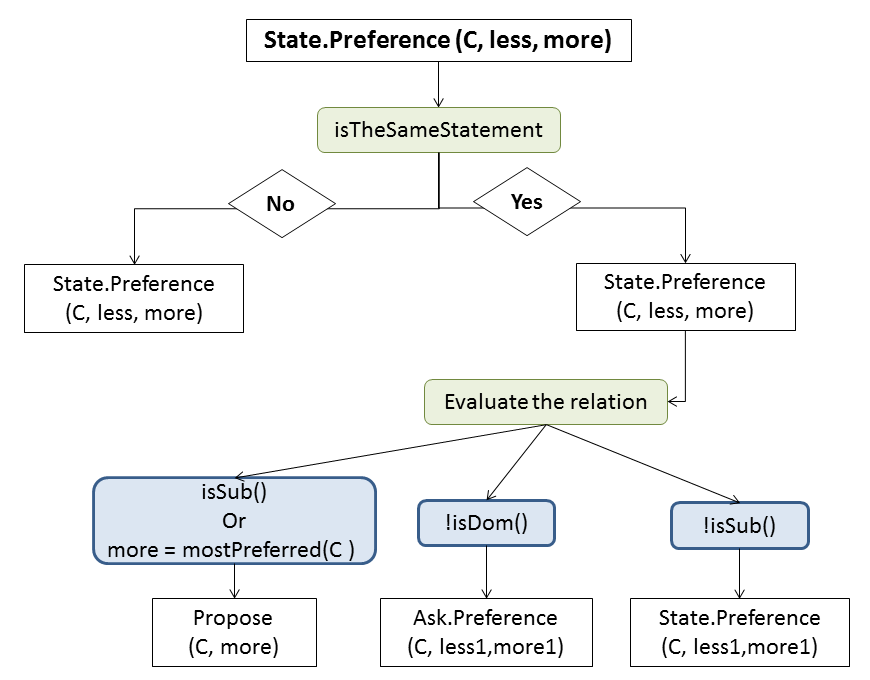
\includegraphics[width=4in]{figs/statePref_v2.png}}
	\vskip 8pt
 	\defig{state}{Les réponses générés suite à un statePreference}
 \end{figure}

\section{Perspectives de recherche}
\label{conc}
Dans cet article, nous avons présenté une architecture de dialogue qui permet à l'agent de mener une négociation coopérative et d'adapter sa stratégie de négociation en fonction de la relation interpersonnelle construite avec l'utilisateur. Nous avons effectué une première implémentation de ce système. 

\par La prochaine étape de nos travaux se concentrera sur l’évaluation d’un tel système de dialogue social. Tout d'abord, nous souhaitons évaluer si le comportement de l'agent durant le dialogue traduit le comportement attendu. Ce type d'évaluation peut s'effectuer à l'aide de tests perceptifs avec les utilisateurs. 
Ensuite, une évaluation du système durant les interactions doit être effectuée où nous cherchons à étudier l'impact des relations sociales sur la qualité du dialogue. Il s’agira alors de vérifier non seulement la perception par l’utilisateur des comportements sociaux de l’agent au cours de l'interaction mais aussi l’effet de tels comportements sur l’engagement de l’utilisateur et la qualité de la négociation menée durant le dialogue. L'hypothèse est que l'interaction est plus agréable avec un agent social et que la négociation sera plus rapide à converger.

\par Outre les perspectives liées à la validation, nous souhaitons réaliser des améliorations sur le système. En effet, nous souhaitons étendre notre système avec un module de théorie de l'esprit. Un tel module permettra à l'agent de comprendre les intentions de l'utilisateur durant la négociation et ainsi, prédire le comportement futur de ce dernier.  De plus, un tel module permettrait d'avoir une meilleure  représentation de la pensée de l'utilisateur et donc une meilleure compréhension de son comportement. Cette connaissance supplémentaire sur l'utilisateur permettrait à l'agent d'avoir une meilleure perception de la relation sociale et ainsi d'adapter efficacement sa stratégie afin de générer une négociation coopérative la plus efficace possible.
%de plus une évaluation avec
%Ajouter un module de théorie de l'esprit afin de de comporendre les intentions communicative de l'utilisateur et ainsi pridir son comportement pour une meilleure négociation. 
%=====================================================================================================
\vskip 4pt
\bibliographystyle{abbrv}
\bibliography{Library}

\end{document}
